\begin{bfseries}
\emph{Abstract} -- 
This paper summarizes our work for the second homework in the course \emph{Control, Theory \& Practice}. 
In this exercise linear models of a four-tank process is investigated for two different settings of the valves (see Figure \ref{tank}).
The first part deals with the analysis of the poles and zeros of the system.
The second part deals with the decentralized control of the system.
\end{bfseries}

\begin{center}
\begin{figure}[h!b]
    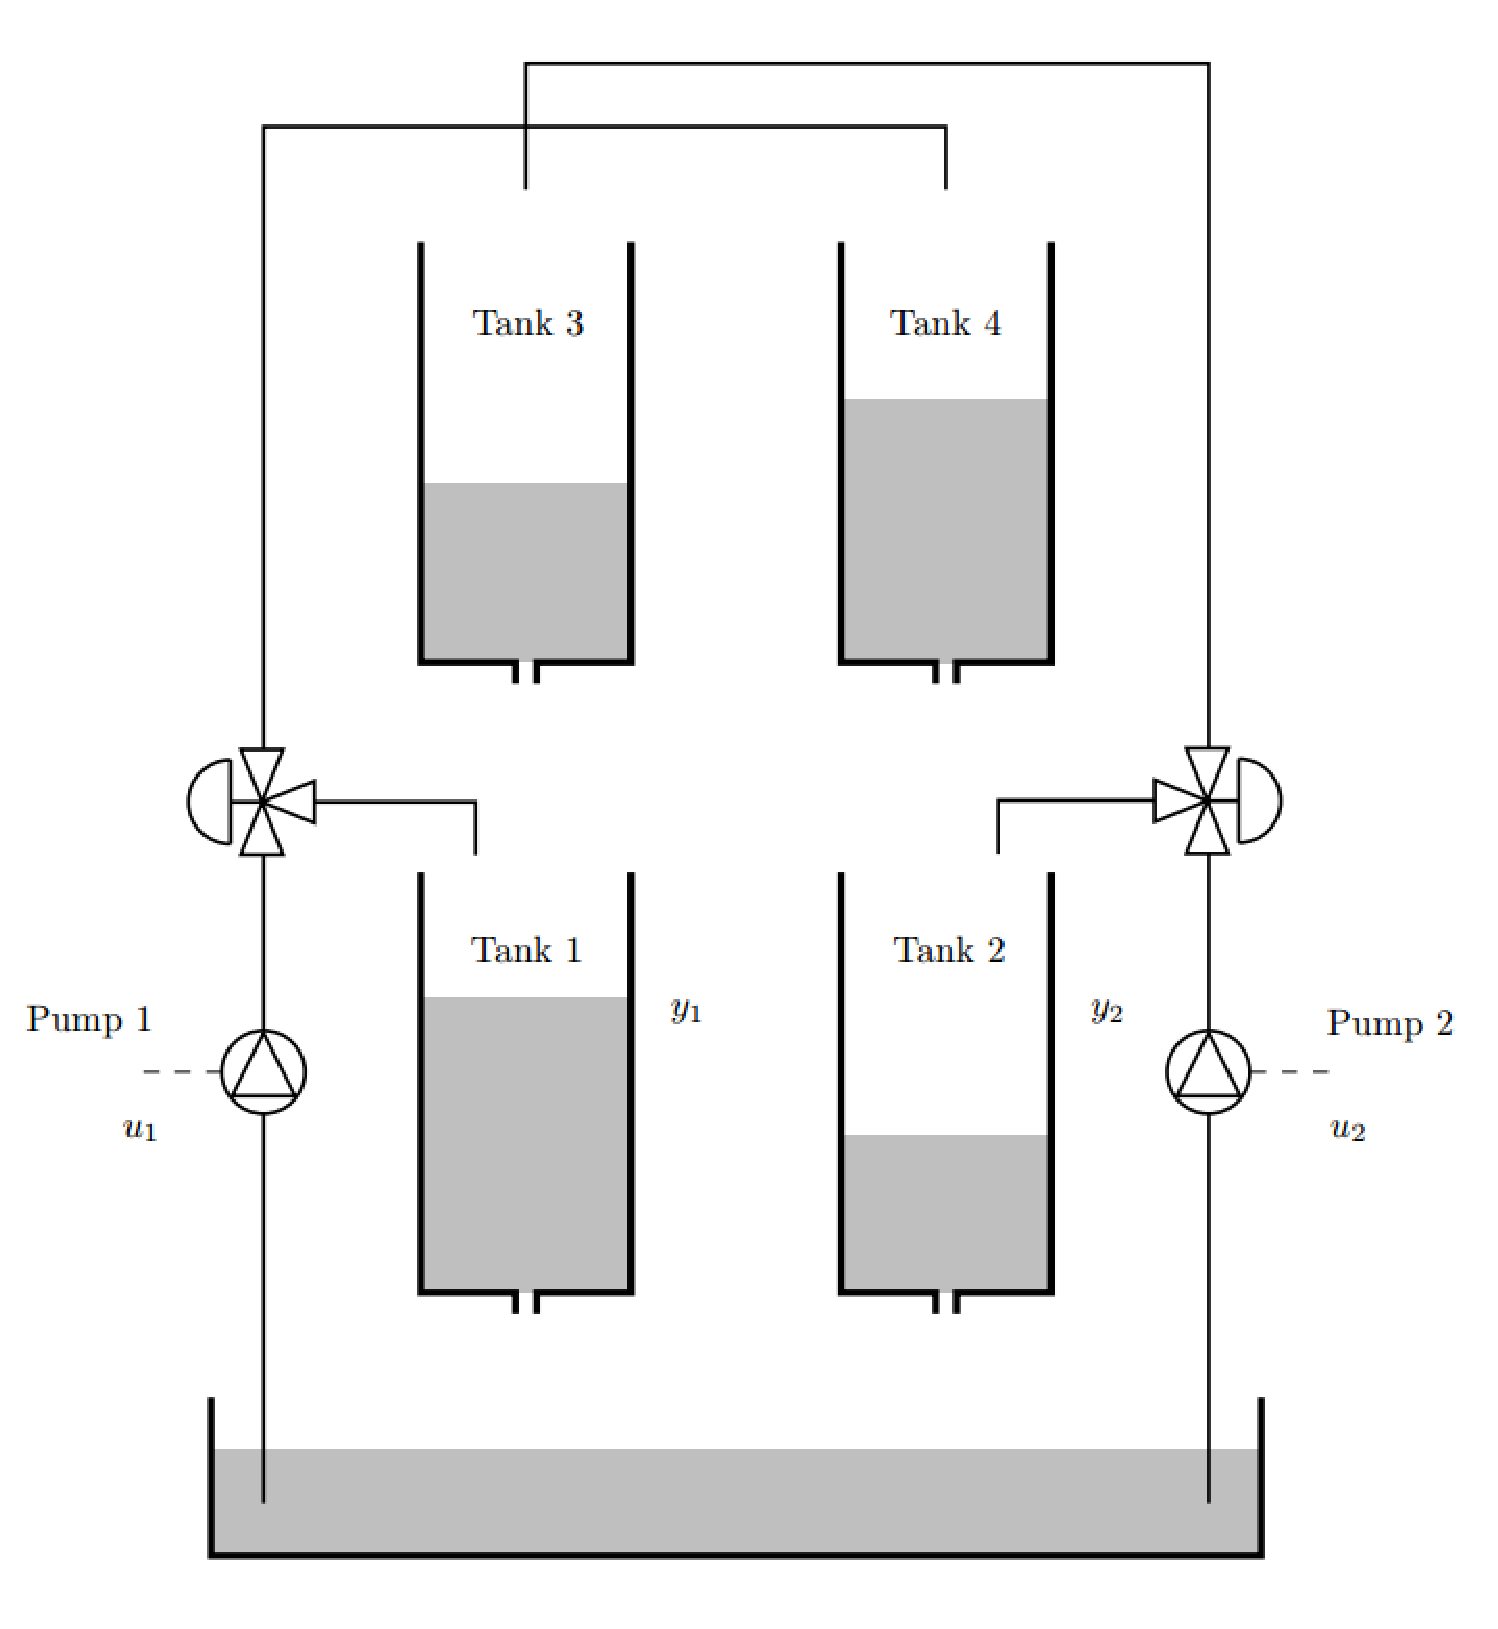
\includegraphics[width=\columnwidth]{fig/tank.eps}
    \caption{The four tank process}
    \label{tank}
\end{figure}
\end{center}
